The method was implemented in C++ using the \texttt{Eigen} library for linear algebra operations \cite{eigen}, particularly for the creation of the sparse matrix $\vf{A}$ described above and the resolution of the resulting linear system using the Cholesky decomposition. We opted not to employ parallelization for the sake of simplicity. However, readers may observe that for achieving more accurate results, such as using a denser grid around the boundary of the object and thereby expanding the size of the discrete domain, parallelization becomes essential\footnote{For further details on the implementation, we shared our code in the Github repository \href{https://github.com/victorballester7/von-karman}{https://github.com/victorballester7/von-karman}. There the reader will also find animations of the flow dynamics around different objects to better understand the phenomenon.}

Implementing the numerical scheme outlined in \cref{sec: diffScheme} we have the opportunity to explore the dynamics of fluid flow around various objects. First, we want to illustrate the emergence of the phenomenon before delving in different factors on the flow as differences in Reynolds numbers or in the shape of the object.

\subsection{Observing von Kármán vortex street}
% Show that we observe the phenomon describe time evolution, how can we see that the periodic state is achieved etc.  What are our needs for dt, dx etc.
%Plot of longterm behaviour for cylidner in flow at two times vorticity, absolute velocity 
To investigate how the phenomenon emerge, we look at an exemplary showcase of a fluid with a Reynolds number $\Rey = 500$. We simulate the fluid in a domain of the width $W = 1$ and the length $L = 5$. For most of the simulations we use a homogeneous grid with 500 grid points in the $x$ direction and 100 grid points in the $y$ direction.
\begin{figure}[!htb]
    \centering
    \hspace*{0.7cm}
    \begin{subfigure}[b]{\linewidth} % Adjust the width as needed
        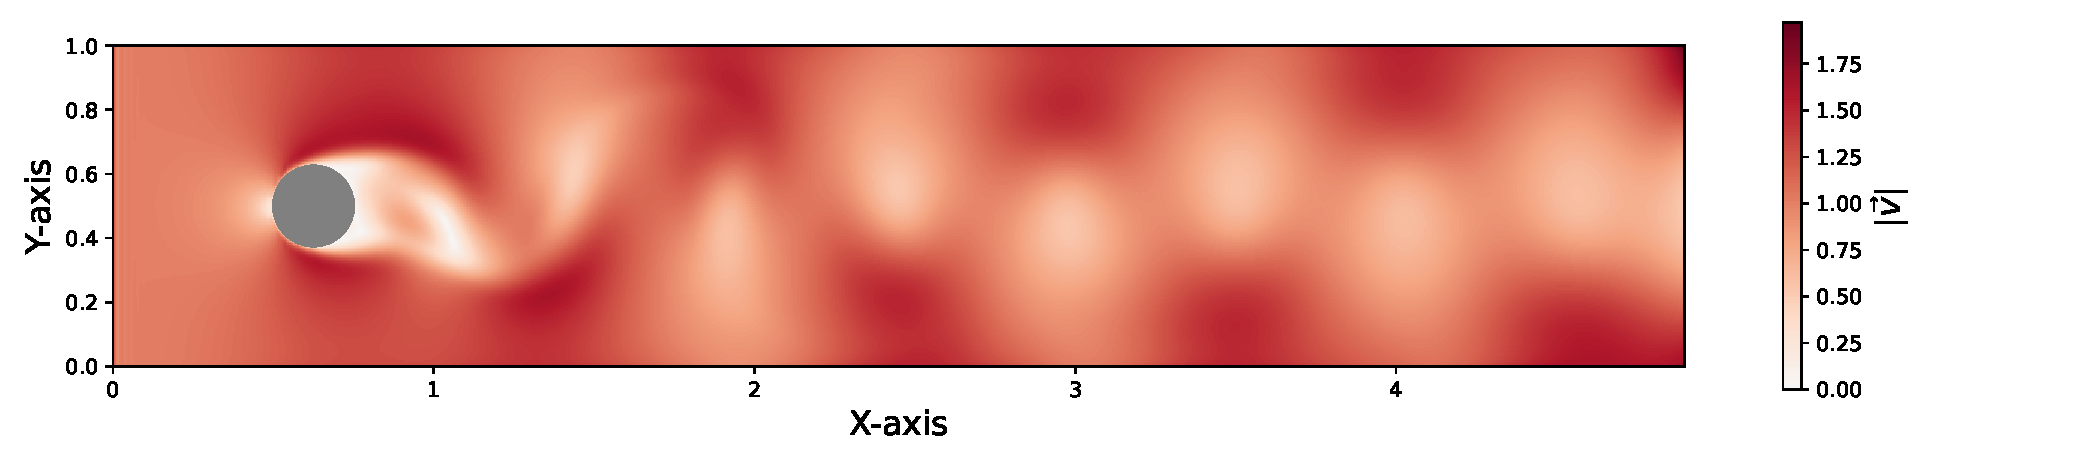
\includegraphics[width=\linewidth]{0_graphics/numeric/absV_25_sim.pdf}
        \caption{Magnitude of the velocity $\sqrt{u^2+v^2}$}
        \label{fig:abs_velocity_25}
    \end{subfigure}
    \vspace{1em} % Adjust space between subfigures as needed
    \hspace*{0.7cm}
    \begin{subfigure}[b]{\linewidth} % Adjust the width as needed
        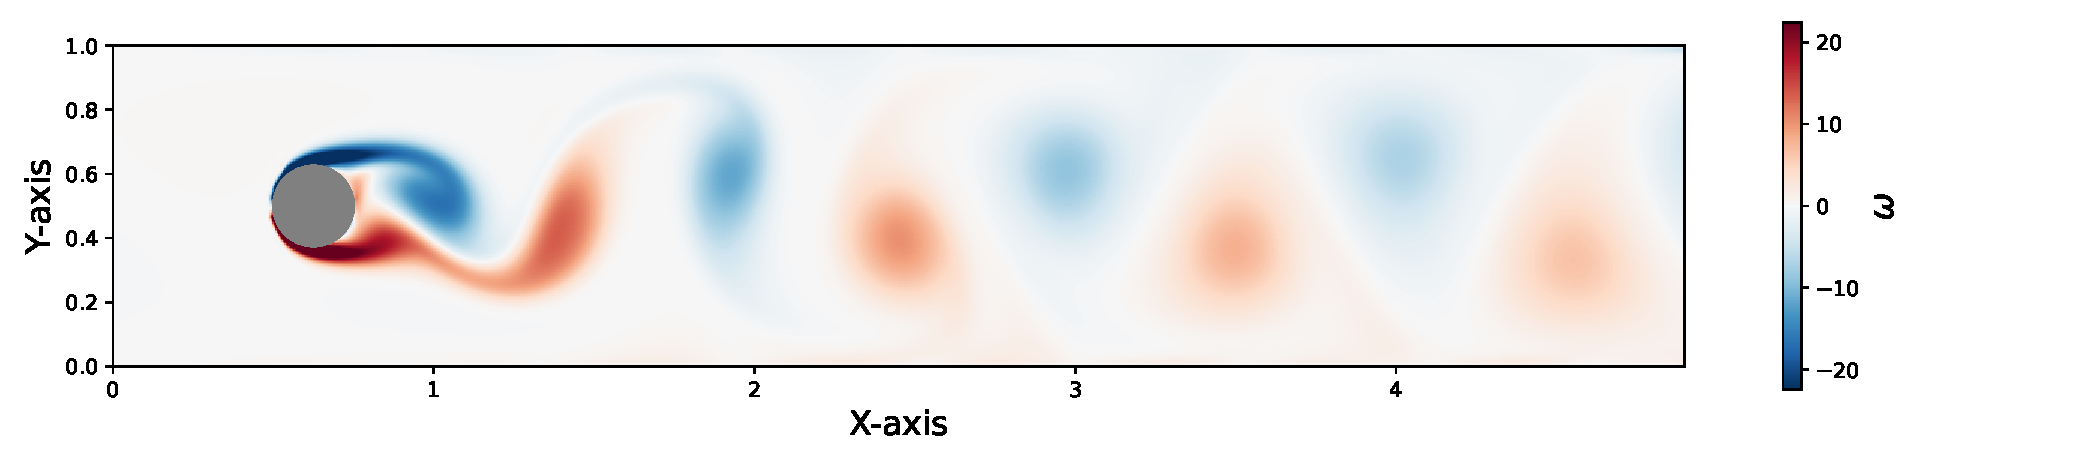
\includegraphics[width=\linewidth]{0_graphics/numeric/vor_25_sim.pdf} % Assuming a different file for vorticity
        \caption{Vorticity $\omega$.}
        \label{fig:vorticity_25}
    \end{subfigure}
    \vspace{-15pt}
    \caption{Flow dynamics around a circular obstacle in a fluid with Reynolds number $\Rey = 500$ at time $t=25$. The top image displays the magnitude of the velocity $\sqrt{u^2+v^2}$, and the bottom image focuses on the vorticity $\omega$.}
    \label{fig:first_karman}
\end{figure}
The time step is taken in an adaptative way, in order to ensure the CFL condition discussed in \cref{sec: diffScheme}. On the right side of the domain we place a circle with radius $r = 0.125$ as an object and at the start of the simulation the fluid inside the domain is at rest. Imposing the boundary conditions as presented in \cref{sec: posingProblem}, the fluid starts to move from the left side to the right side of the domain.
As the simulation progresses, the flow dynamics evolve to reveal the organized structure known as a von Kármán vortex street. In \cref{fig:first_karman}, we present the outcomes of this prolonged simulation, showcasing the magnitude of the velocity field and the vorticity $ \omega=\nabla \times \vf{u} = \frac{\partial v}{\partial x} - \frac{\partial u}{\partial y}$, to visualize the vortices. The vorticity measures the local rotation of the velocity field. In the figure we can observe the characteristic periodicity between red (counterclockwise rotating vortices) and blue (clockwise rotating vortices) vortices. In front of the body the flow seems to be laminar with an income velocity of approximately $u = 1$ (after normalization), which is consistent with our boundary conditions.



\subsection{Influence of Reynolds number}
% Analysis how high low reynoldsnumber influence the flow and the phenomenon Maybe there is a limit for our solver or there is a limit for the phenomenon 
The Reynolds number plays an important role in determining the flow characteristics around bodies in a fluid. It serves as a crucial indicator for the flow regime around bodies immersed in a fluid, significantly influencing the resulting flow patterns. In this section, we look at the same setup as before and vary the Reynolds number. The impact can be categorized in different regimes. In \cref{fig:influenceRey1} we plot the vorticity of the flow for different Reynolds numbers. 

\begin{figure}[!htb]
    \centering
    \hspace*{0.7cm}
    \begin{subfigure}[b]{\linewidth} % Adjust the width as needed
        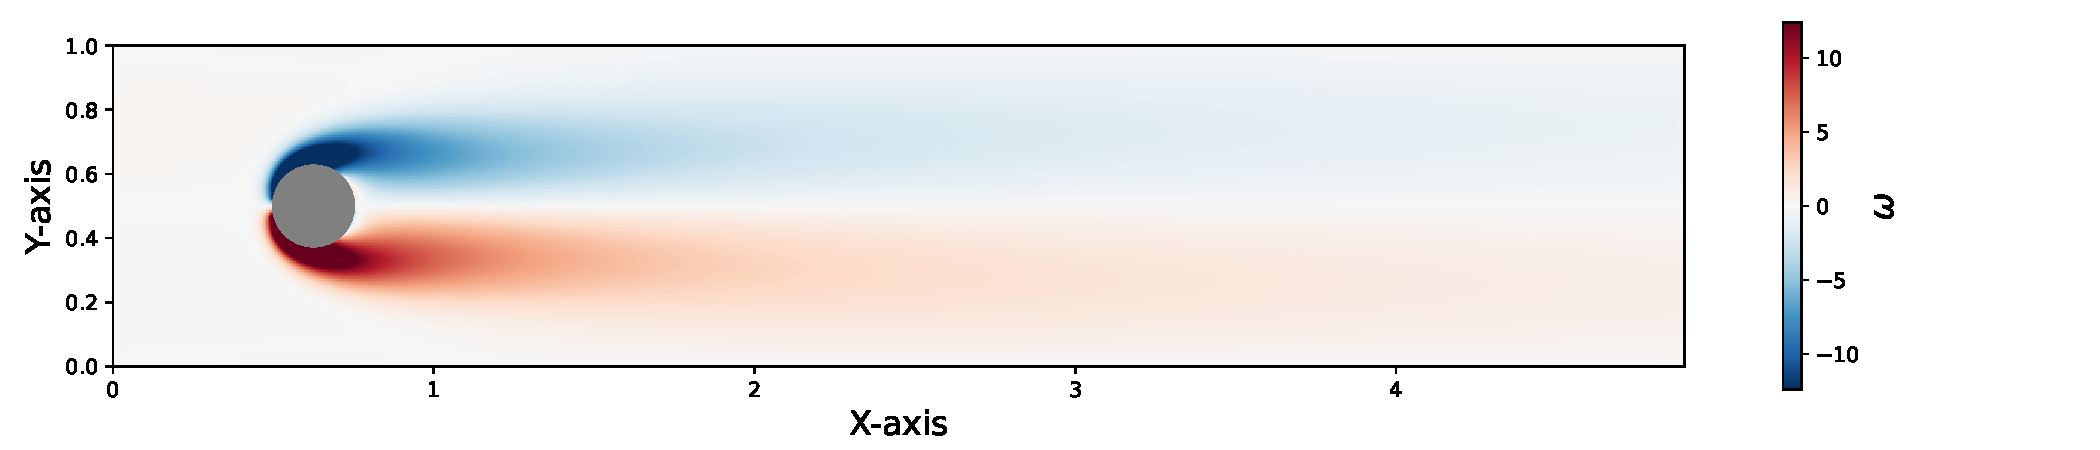
\includegraphics[width=\linewidth]{0_graphics/numeric/RE100_30_sim.pdf}
        \caption{Vorticity $\omega$ for $\Rey = 100$}
        \label{fig:RE100_vor_40}
    \end{subfigure}

    \hspace*{0.7cm}
    \begin{subfigure}[b]{\linewidth} % Adjust the width as needed
        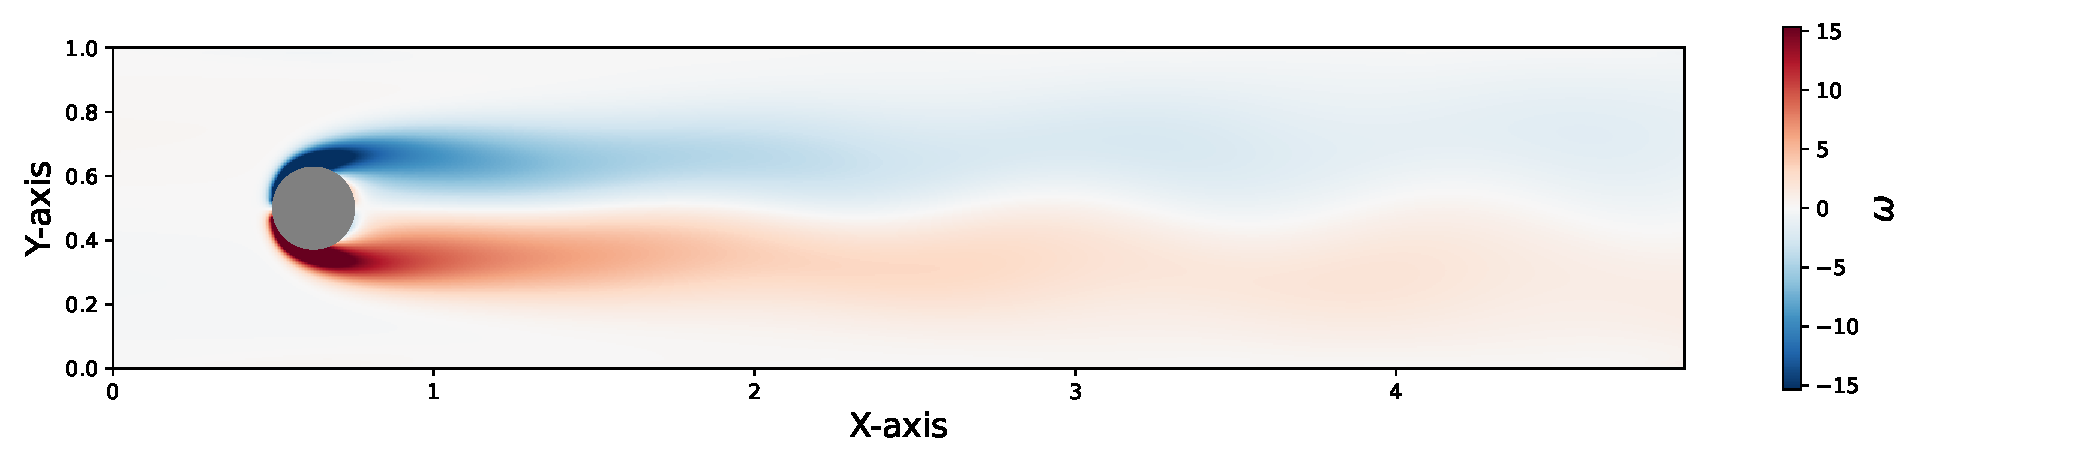
\includegraphics[width=\linewidth]{0_graphics/numeric/RE175_30_sim.pdf}
        \caption{Vorticity $\omega$ for $\Rey = 175$}
        \label{fig:RE175_vor_40}
    \end{subfigure}

        \hspace*{0.7cm}
    \begin{subfigure}[b]{\linewidth} % Adjust the width as needed
        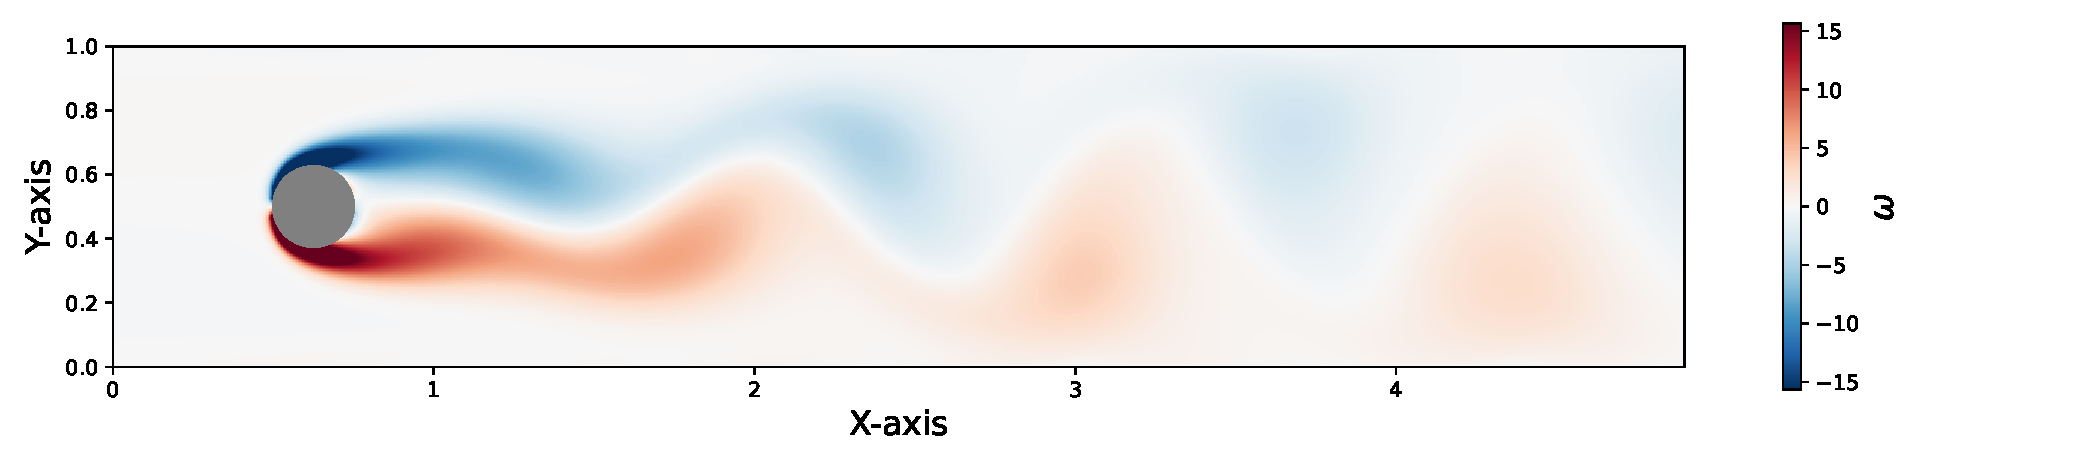
\includegraphics[width=\linewidth]{0_graphics/numeric/RE190_30_sim.pdf}
        \caption{Vorticity $\omega$ for $\Rey = 190$}
        \label{fig:RE190_vor_40}
    \end{subfigure}

        \hspace*{0.7cm}
    \begin{subfigure}[b]{\linewidth} % Adjust the width as needed
        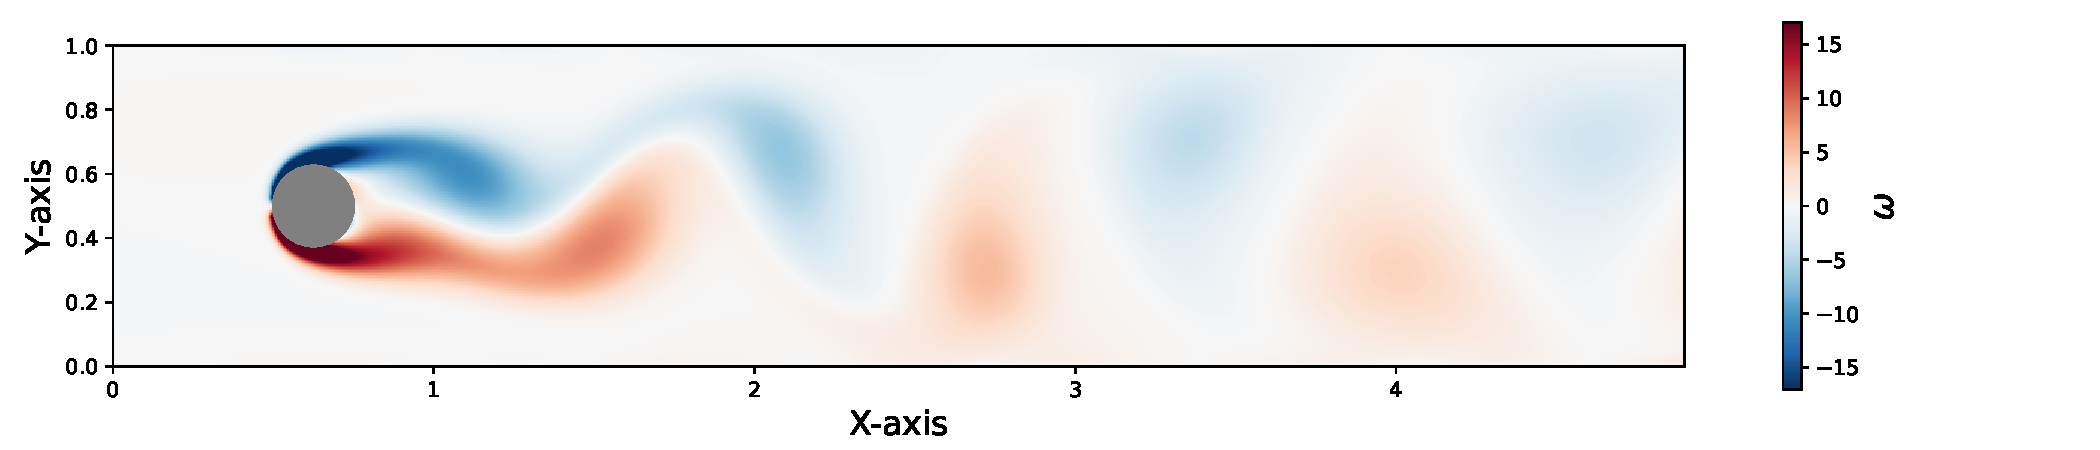
\includegraphics[width=\linewidth]{0_graphics/numeric/RE230_30_sim.pdf} 
        \caption{Vorticity $\omega$ for $\Rey = 230$}
        \label{fig:RE230_vor_40}
    \end{subfigure}

    \vspace{-5pt}
    \caption{Flow dynamics around a circular obstacle for fluid with different Reynolds numbers at time $t=30$.}
    \label{fig:influenceRey1}
\end{figure}

The impact of the Reynolds number is evident. For low Reynolds numbers ($\Rey \leq 150$) the flow stays laminar, and pattern formation is not observed. For $\Rey \approx 175$ the flow starts to be more complex. We don't observe vortices, but behind the body the vertical velocity periodically changes. Increasing the Reynolds number further we observe that the periodic perturbation become stronger ($\Rey = 190$), until finally vortices emerge ($\Rey \geq 230$).


\subsection{Influence of the object}
We this section we aim to demonstrate the impact of object geometry on the flow characteristics. To show that the geometry of objects immersed in a fluid significantly influences the flow patterns that develop around them, we look at a more advanced shape: an airfoil. This shape is not just designed to create lift for a plane, but also to ensure that the flow patterns are stable and manageable. This stability is essential for effective maneuverability during flight.

\begin{figure}[!htb]
    \centering
    \hspace*{0.7cm}
    \begin{subfigure}[b]{\linewidth} % Adjust the width as needed
        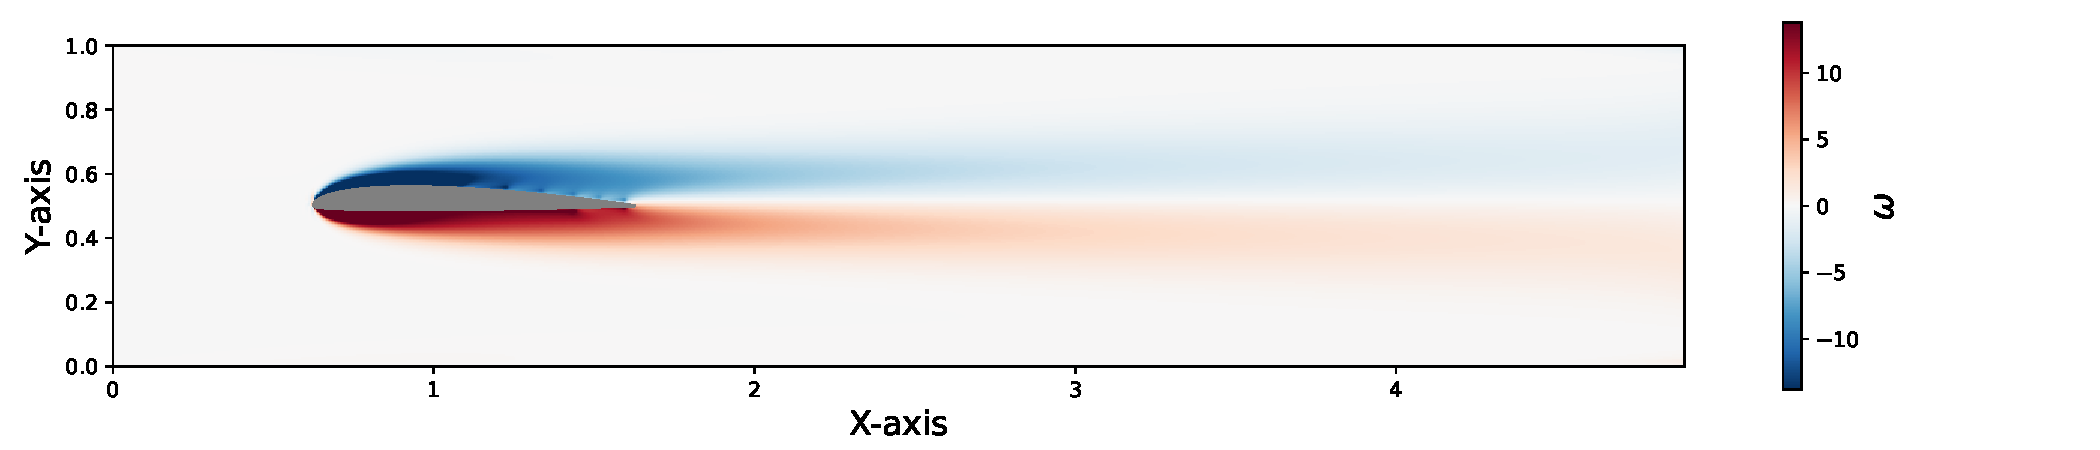
\includegraphics[width=\linewidth]{0_graphics/numeric/RE500_30_airfoil.pdf}
        \caption{Vorticity $\omega$ for $\Rey = 500$}
        \label{fig:RE500_airfoil}
    \end{subfigure}

    \hspace*{0.7cm}
    \begin{subfigure}[b]{\linewidth} % Adjust the width as needed
        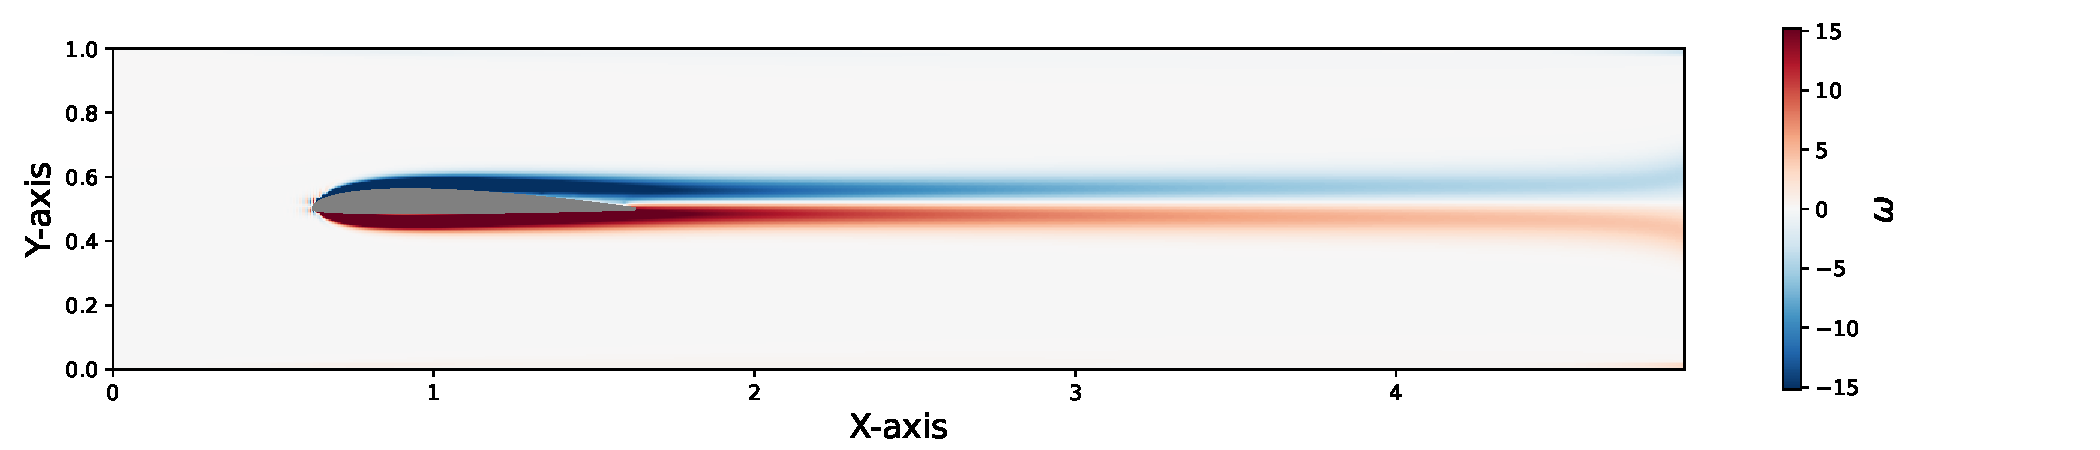
\includegraphics[width=\linewidth]{0_graphics/numeric/RE3500_30_airfoil.pdf}
        \caption{Vorticity $\omega$ for $\Rey = 3500$}
        \label{fig:RE3500_airfoil}
    \end{subfigure}

    \hspace*{0.7cm}
    \begin{subfigure}[b]{\linewidth} % Adjust the width as needed
        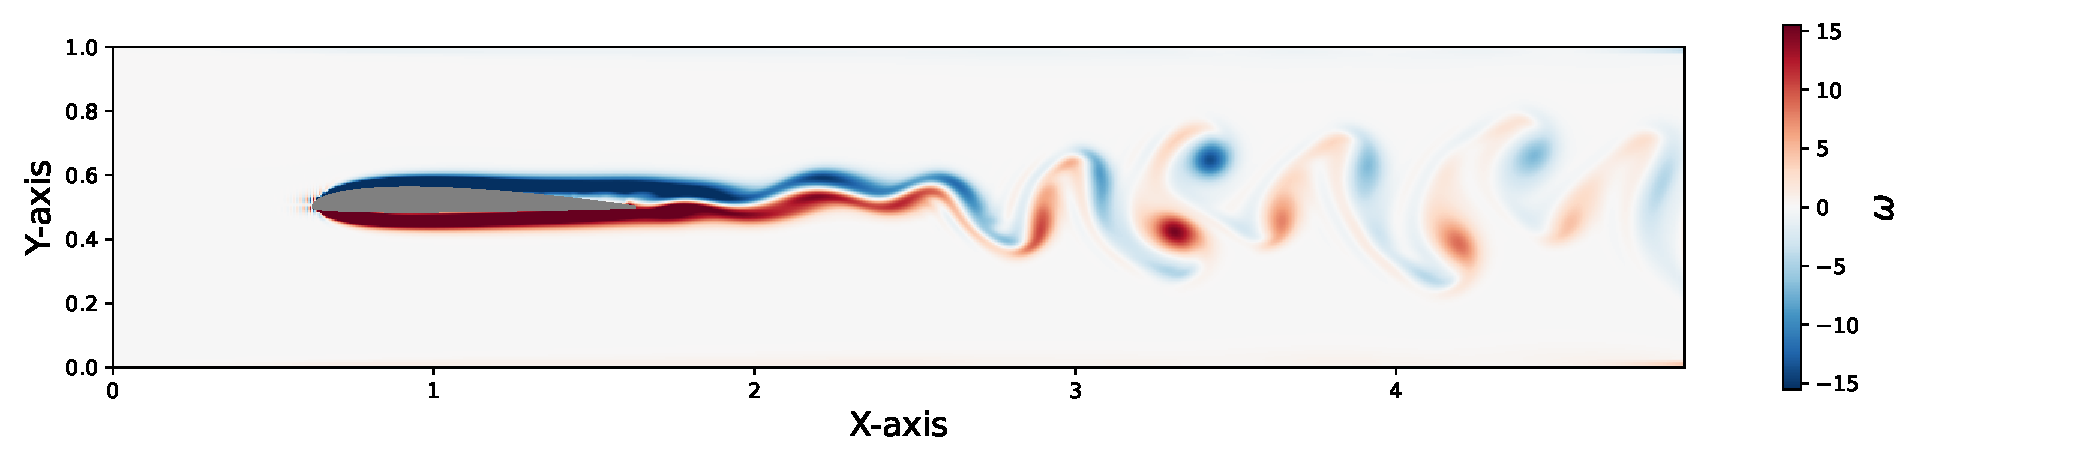
\includegraphics[width=\linewidth]{0_graphics/numeric/RE5500_30_airfoil.pdf}
        \caption{Vorticity $\omega$ for $\Rey = 5500$}
        \label{fig:RE5500_airfoil}
    \end{subfigure}

    \caption{Flow dynamics around an airfoil in a fluid with different Reynolds numbers at time $t=30$.}
    \label{fig:airfoil}
\end{figure}

In \cref{fig:RE500_airfoil}, we present our findings for the airfoil subjected to a Reynolds number $\Rey = 500$. In contrast with the observations made in \cref{fig:abs_velocity_25} for the circle, the flow surrounding the airfoil is remarkably devoid of vortices or significant flow perturbations. The elongated shape reduces the region in which the side eddies can interact and delays the onset of mixing to a position much farther behind the object. This difference demonstrates the influence of object geometry on flow dynamics. The streamlined shape of the airfoil leads to smoother flow, reducing the tendency for vortex formation.

It is important to note that comparing flows around bodies of dissimilar shapes at equivalent Reynolds numbers is inherently challenging. This challenge arises due to the variability in characteristic lengths and velocities, which fundamentally alters the flow's nature around each object. But even increasing the Reynolds number to $\Rey=3500$, does not lead to turbulences in the flow. As we can see in \cref{fig:RE3500_airfoil} the flow around the airfoil maintains a predominantly laminar characteristic, a testament to its aerodynamically efficient design. 

Only when we further increase the Reynolds number to $\Rey=5500$, the flow around the airfoil begins to exhibit clear signs of turbulence, marked by the formation of vortices. In \cref{fig:RE5500_airfoil} we plot the results and we can clearly see vortices arising behind the foil. The circle, with its inherent propensity to induce turbulence, resulted in flow conditions too chaotic for our solver to accurately simulate over extended durations. 

In the case of the airfoil we see that the influence of the shape on flow dynamics is very important. This underscores the significance of the complexity in designing aircraft that must operate effectively across a broad range of speeds. As a result, the design of wings is not only highly optimized but, in certain cases, incorporates the ability to change shape dynamically to adapt optimally to the aircraft's velocity.